\chapter{Todennäköisyys}

\index{todennxkzisyys@todennäköisyys}

\key{Todennäköisyys} on luku väliltä $0 \ldots 1$,
joka kuvaa sitä, miten todennäköinen jokin
tapahtuma on.
Varman tapahtuman todennäköisyys on 1,
ja mahdottoman tapahtuman todennäköisyys on 0.

Tyypillinen esimerkki todennäköisyydestä
on nopan heitto, jossa tuloksena
on silmäluku väliltä $1,2,\ldots,6$.
Yleensä oletetaan, että kunkin silmäluvun
todennäköisyys on $1/6$
eli kaikki tulokset ovat yhtä todennäköisiä.

Tapahtuman todennäköisyyttä merkitään $P(\cdots)$,
jossa kolmen pisteen tilalla on tapahtuman kuvaus.
Esimerkiksi nopan heitossa
$P(\textrm{''silmäluku on 4''})=1/6$,
$P(\textrm{''silmäluku ei ole 6''})=5/6$
ja $P(\textrm{''silmäluku on parillinen''})=1/2$.

\section{Laskutavat}

Todennäköisyyden laskemiseen on kaksi
tavallista laskutapaa:
kombinatorinen laskeminen ja prosessin simulointi.
Lasketaan esimerkkinä, mikä on todennäköisyys sille,
että kun sekoitetusta korttipakasta nostetaan
kolme ylintä korttia, jokaisen kortin arvo on sama
(esimerkiksi ristikasi, herttakasi ja patakasi).

\subsubsection*{Laskutapa 1}

Kombinatorisessa laskutavassa
todennäköisyyden kaava on

\[\frac{\textrm{halutut tapaukset}}{\textrm{kaikki tapaukset}}.\]

Tässä tehtävässä halutut tapaukset ovat niitä,
joissa jokaisen kolmen kortin arvo on sama.
Tällaisia tapauksia on $13 {4 \choose 3}$,
koska on 13 vaihtoehtoa, mikä on kortin arvo,
ja ${4 \choose 3}$ tapaa valita 3 maata 4 mahdollisesta.

Kaikkien tapausten määrä on ${52 \choose 3}$,
koska 52 kortista valitaan 3 korttia.
Niinpä tapahtuman todennäköisyys on

\[\frac{13 {4 \choose 3}}{{52 \choose 3}} = \frac{1}{425}.\]

\subsubsection*{Laskutapa 2}

Toinen tapa laskea todennäköisyys on simuloida prosessia,
jossa tapahtuma syntyy.
Tässä tapauksessa pakasta nostetaan kolme korttia,
joten prosessissa on kolme vaihetta.
Vaatimuksena on, että prosessin jokainen vaihe onnistuu.

Ensimmäisen kortin nosto onnistuu varmasti,
koska mikä tahansa kortti kelpaa.
Tämän jälkeen kahden seuraavan kortin
arvon tulee olla sama.
Toisen kortin nostossa kortteja on jäljellä 51
ja niistä 3 kelpaa, joten todennäköisyys on $3/51$.
Vastaavasti kolmannen kortin nostossa
todennäköisyys on $2/50$.

Todennäköisyys koko prosessin onnistumiselle on

\[1 \cdot \frac{3}{51} \cdot \frac{2}{50} = \frac{1}{425}.\]

\section{Tapahtumat}

Todennäköisyyden tapahtuma
voidaan esittää joukkona
\[A \subset X,\]
missä $X$ sisältää kaikki mahdolliset alkeistapaukset
ja $A$ on jokin alkeistapausten osajoukko.
Esimerkiksi nopanheitossa alkeistapaukset ovat
\[X = \{x_1,x_2,x_3,x_4,x_5,x_6\},\]
missä $x_k$ tarkoittaa silmälukua $k$.
Nyt esimerkiksi tapahtumaa ''silmäluku on parillinen''
vastaa joukko
\[A = \{x_2,x_4,x_6\}.\]

Jokaista alkeistapausta $x$
vastaa todennäköisyys $p(x)$.
Tämän ansiosta joukkoa $A$ vastaavan tapahtuman
todennäköisyys $P(A)$ voidaan
laskea alkeistapausten todennäköisyyksien
summana kaavalla
\[P(A) = \sum_{x \in A} p(x).\]
Esimerkiksi nopanheitossa $p(x)=1/6$
jokaiselle alkeistapaukselle $x$, joten
tapahtuman ''silmäluku on parillinen''
todennäköisyys on
\[p(x_2)+p(x_4)+p(x_6)=1/2.\]

Alkeistapahtumat tulee aina valita niin,
että kaikkien alkeistapausten
todennäköisyyksien summa on 1 eli $P(X)=1$.

Koska todennäköisyyden tapahtumat ovat joukkoja,
niihin voi soveltaa jouk\-ko-opin operaatioita:

\begin{itemize}
\item \key{Komplementti} $\bar A$ tarkoittaa
tapahtumaa ''$A$ ei tapahdu''. 
Esimerkiksi nopanheitossa tapahtuman
$A=\{x_2,x_4,x_6\}$ komplementti on
$\bar A = \{x_1,x_3,x_5\}$.
\item \key{Yhdiste} $A \cup B$ tarkoittaa
tapahtumaa ''$A$ tai $B$ tapahtuu''.
Esimerkiksi tapahtumien $A=\{x_2,x_5\}$
ja $B=\{x_4,x_5,x_6\}$ yhdiste on
$A \cup B = \{x_2,x_4,x_5,x_6\}$.
\item \key{Leikkaus} $A \cap B$ tarkoittaa
tapahtumaa ''$A$ ja $B$ tapahtuvat''.
Esimerkiksi tapahtumien $A=\{x_2,x_5\}$
ja $B=\{x_4,x_5,x_6\}$ leikkaus on
$A \cap B = \{x_5\}$.
\end{itemize}

\subsubsection{Komplementti}

Komplementin $\bar A$
todennäköisyys lasketaan kaavalla
\[P(\bar A)=1-P(A).\]

Joskus tehtävän ratkaisu on kätevää
laskea komplementin kautta
miettimällä tilannetta käänteisesti.
Esimerkiksi todennäköisyys saada
silmäluku 6 ainakin kerran,
kun noppaa heitetään kymmenen kertaa, on
\[1-(5/6)^{10}.\]

Tässä $5/6$ on todennäköisyys,
että yksittäisen heiton silmäluku ei ole 6,
ja $(5/6)^{10}$ on todennäköisyys, että yksikään
silmäluku ei ole 6 kymmenessä heitossa.
Tämän komplementti tuottaa halutun tuloksen.

\subsubsection{Yhdiste}

Yhdisteen $A \cup B$ todennäköisyys lasketaan kaavalla 
\[P(A \cup B)=P(A)+P(B)-P(A \cap B).\]
Esimerkiksi nopanheitossa tapahtumien
\[A=\textrm{''silmäluku on parillinen''}\]
ja
\[B=\textrm{''silmäluku on alle 4''}\]
yhdisteen
\[A \cup B=\textrm{''silmäluku on parillinen tai alle 4''}\]
todennäköisyys on
\[P(A \cup B) = P(A)+P(B)-P(A \cap B)=1/2+1/2-1/6=5/6.\]

Jos tapahtumat $A$ ja $B$ ovat \key{erilliset} eli $A \cap B$ on tyhjä,
yhdisteen $A \cup B$ todennäköisyys on yksinkertaisesti

\[P(A \cup B)=P(A)+P(B).\]

\subsubsection{Ehdollinen todennäköisyys}

\index{ehdollinen todennxkzisyys@ehdollinen todennäköisyys}

\key{Ehdollinen todennäköisyys}
\[P(A | B) = \frac{P(A \cap B)}{P(B)}\]
on tapahtuman $A$ todennäköisyys
olettaen, että tapahtuma $B$ tapahtuu.
Tällöin todennäköisyyden laskennassa otetaan
huomioon vain ne alkeistapaukset,
jotka kuuluvat joukkoon $B$.

Äskeisen esimerkin joukkoja käyttäen
\[P(A | B)= 1/3,\]
koska joukon $B$ alkeistapaukset ovat
$\{x_1,x_2,x_3\}$ ja niistä yhdessä
silmäluku on parillinen.
Tämä on todennäköisyys saada parillinen silmäluku,
jos tiedetään, että silmäluku on välillä 1--3.

\subsubsection{Leikkaus}

\index{riippumattomuus@riippumattomuus}

Ehdollisen todennäköisyyden avulla
leikkauksen $A \cap B$ todennäköisyys
voidaan laskea kaavalla
\[P(A \cap B)=P(A)P(B|A).\]
Tapahtumat $A$ ja $B$ ovat \key{riippumattomat}, jos
\[P(A|B)=P(A) \hspace{10px}\textrm{ja}\hspace{10px} P(B|A)=P(B),\]
jolloin $B$:n tapahtuminen ei vaikuta $A$:n
todennäköisyyteen ja päinvastoin.
Tässä tapauksessa leikkauksen
todennäköisyys on
\[P(A \cap B)=P(A)P(B).\]
Esimerkiksi pelikortin nostamisessa
tapahtumat
\[A = \textrm{''kortin maa on risti''}\]
ja
\[B = \textrm{''kortin arvo on 4''}\]
ovat riippumattomat.
Niinpä tapahtuman
\[A \cap B = \textrm{''kortti on ristinelonen''}\]
todennäköisyys on
\[P(A \cap B)=P(A)P(B)=1/4 \cdot 1/13 = 1/52.\]

\section{Satunnaismuuttuja}

\index{satunnaismuuttuja@satunnaismuuttuja}

\key{Satunnaismuuttuja} on arvo, joka syntyy satunnaisen
prosessin tuloksena.
Satunnaismuuttujaa merkitään yleensä
suurella kirjaimella.
Esimerkiksi kahden nopan heitossa yksi mahdollinen
satunnaismuuttuja on
\[X=\textrm{''silmälukujen summa''}.\]
Esimerkiksi jos heitot ovat $(4,6)$,
niin $X$ saa arvon 10.

Merkintä $P(X=x)$ tarkoittaa todennäköisyyttä,
että satunnaismuuttujan $X$ arvo on $x$.
Edellisessä esimerkissä $P(X=10)=3/36$,
koska erilaisia heittotapoja on 36
ja niistä summan 10 tuottavat heitot
$(4,6)$, $(5,5)$ ja $(6,4)$.

\subsubsection{Odotusarvo}

\index{odotusarvo@odotusarvo}

\key{Odotusarvo} $E[X]$ kertoo, mikä satunnaismuuttujan $X$
arvo on keskimääräisessä tilanteessa.
Odotusarvo lasketaan summana
\[\sum_x P(X=x)x,\]
missä $x$ saa kaikki mahdolliset satunnaismuuttujan arvot.

Esimerkiksi nopan heitossa silmäluvun odotusarvo on

\[1/6 \cdot 1 + 1/6 \cdot 2 + 1/6 \cdot 3 + 1/6 \cdot 4 + 1/6 \cdot 5 + 1/6 \cdot 6 = 7/2.\]

Usein hyödyllinen odotusarvon ominaisuus on \key{lineaarisuus}.
Sen ansiosta summa $E[X_1+X_2+\cdots+X_n]$ voidaan laskea $E[X_1]+E[X_2]+\cdots+E[X_n]$.
Kaava pätee myös silloin, kun satunnaismuuttujat riippuvat toisistaan.

Esimerkiksi kahden nopan heitossa silmälukujen summan odotusarvo on
\[E[X_1+X_2]=E[X_1]+E[X_2]=7/2+7/2=7.\]

Tarkastellaan sitten tehtävää,
jossa $n$ laatikkoon sijoitetaan
satunnaisesti $n$ palloa
ja laskettavana on odotusarvo,
montako laatikkoa jää tyhjäksi.
Kullakin pallolla on yhtä suuri todennäköisyys
päätyä mihin tahansa laatikkoon.
Esimerkiksi jos $n=2$, niin
vaihtoehdot ovat seuraavat:
\begin{center}
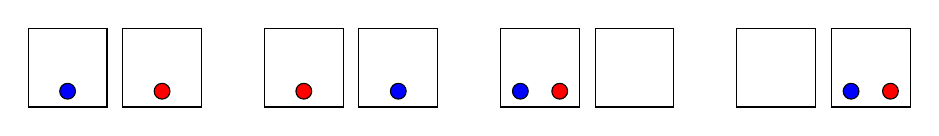
\begin{tikzpicture}
\draw (0,0) rectangle (1,1);
\draw (1.2,0) rectangle (2.2,1);
\draw (3,0) rectangle (4,1);
\draw (4.2,0) rectangle (5.2,1);
\draw (6,0) rectangle (7,1);
\draw (7.2,0) rectangle (8.2,1);
\draw (9,0) rectangle (10,1);
\draw (10.2,0) rectangle (11.2,1);

\draw[fill=blue] (0.5,0.2) circle (0.1);
\draw[fill=red] (1.7,0.2) circle (0.1);
\draw[fill=red] (3.5,0.2) circle (0.1);
\draw[fill=blue] (4.7,0.2) circle (0.1);
\draw[fill=blue] (6.25,0.2) circle (0.1);
\draw[fill=red] (6.75,0.2) circle (0.1);
\draw[fill=blue] (10.45,0.2) circle (0.1);
\draw[fill=red] (10.95,0.2) circle (0.1);
\end{tikzpicture}
\end{center}
Tässä tapauksessa odotusarvo
tyhjien laatikoiden määrälle on
\[\frac{0+0+1+1}{4} = \frac{1}{2}.\]
Yleisessä tapauksessa
todennäköisyys, että yksittäinen laatikko on tyhjä,
on
\[\Big(\frac{n-1}{n}\Big)^n,\]
koska mikään pallo ei saa mennä sinne.
Niinpä odotusarvon lineaarisuuden ansiosta tyhjien laatikoiden
määrän odotusarvo on
\[n \cdot \Big(\frac{n-1}{n}\Big)^n.\]

\subsubsection{Jakaumat}

\index{jakauma@jakauma}

Satunnaismuuttujan \key{jakauma} kertoo,
millä todennäköisyydellä satunnaismuuttuja
saa minkäkin arvon.
Jakauma muodostuu arvoista $P(X=x)$.
Esimerkiksi kahden nopan heitossa
silmälukujen summan jakauma on:
\begin{center}
\small {
\begin{tabular}{r|rrrrrrrrrrrrr}
$x$ & 2 & 3 & 4 & 5 & 6 & 7 & 8 & 9 & 10 & 11 & 12 \\
$P(X=x)$ & $1/36$ & $2/36$ & $3/36$ & $4/36$ & $5/36$ & $6/36$ & $5/36$ & $4/36$ & $3/36$ & $2/36$ & $1/36$ \\
\end{tabular}
}
\end{center}
Tutustumme seuraavaksi muutamaan usein esiintyvään jakaumaan.
\index{tasajakauma@tasajakauma}
~\\\\
\key{Tasajakauman} satunnaismuuttuja
saa arvoja väliltä $a \ldots b$
ja jokaisen arvon todennäköisyys on sama.
Esimerkiksi yhden nopan heitto tuottaa tasajakauman,
jossa $P(X=x)=1/6$, kun $x=1,2,\ldots,6$.

Tasajakaumassa $X$:n odotusarvo on
\[E[X] = \frac{a+b}{2}.\]
\index{binomijakauma@binomijakauma}
~\\
\key{Binomijakauma} kuvaa tilannetta, jossa tehdään $n$
yritystä ja joka yrityksessä onnistumisen
todennäköisyys on $p$. Satunnaismuuttuja $X$
on onnistuneiden yritysten määrä,
ja arvon $x$ todennäköisyys on
\[P(X=x)=p^x (1-p)^{n-x} {n \choose x},\]
missä $p^x$ kuvaa onnistuneita yrityksiä,
$(1-p)^{n-x}$ kuvaa epäonnistuneita yrityksiä
ja ${n \choose x}$ antaa erilaiset tavat,
miten yritykset sijoittuvat toisiinsa nähden.

Esimerkiksi jos heitetään 10 kertaa noppaa,
todennäköisyys saada tarkalleen 3 kertaa silmäluku 6
on $(1/6)^3 (5/6)^7 {10 \choose 3}$.

Binomijakaumassa $X$:n odotusarvo on
\[E[X] = pn.\]
\index{geometrinen jakauma@geometrinen jakauma}
~\\
\key{Geometrinen jakauma} kuvaa tilannetta,
jossa onnistumisen todennäköisyys on $p$
ja yrityksiä tehdään, kunnes tulee ensimmäinen
onnistuminen. Satunnaismuuttuja $X$ on
tarvittavien yritysten määrä,
ja arvon $x$ todennäköisyys on
\[P(X=x)=(1-p)^{x-1} p,\]
missä $(1-p)^{x-1}$ kuvaa epäonnistuneita yrityksiä ja
$p$ on ensimmäinen onnistunut yritys.

Esimerkiksi jos heitetään noppaa,
kunnes tulee silmäluku 6, todennäköisyys
heittää tarkalleen 4 kertaa on $(5/6)^3 1/6$.

Geometrisessa jakaumassa $X$:n odotusarvo on
\[E[X]=\frac{1}{p}.\]

\section{Markovin ketju}

\index{Markovin ketju@Markovin ketju}

\key{Markovin ketju} on satunnaisprosessi,
joka muodostuu tiloista ja niiden välisistä siirtymistä.
Jokaisesta tilasta tiedetään, millä todennäköisyydellä
siitä siirrytään toisiin tiloihin.
Markovin ketju voidaan esittää verkkona,
jonka solmut ovat tiloja
ja kaaret niiden välisiä siirtymiä.

Tarkastellaan esimerkkinä tehtävää,
jossa olet alussa $n$-kerroksisen
rakennuksen kerroksessa 1.
Joka askeleella liikut satunnaisesti
kerroksen ylöspäin tai alaspäin,
paitsi kerroksesta 1 liikut aina ylöspäin
ja kerroksesta $n$ aina alaspäin.
Mikä on todennäköisyys, että olet $m$
askeleen jälkeen kerroksessa $k$?

Tehtävässä kukin rakennuksen kerros
on yksi tiloista, ja kerrosten välillä liikutaan
satunnaisesti.
Esimerkiksi jos $n=5$, verkosta tulee:

\begin{center}
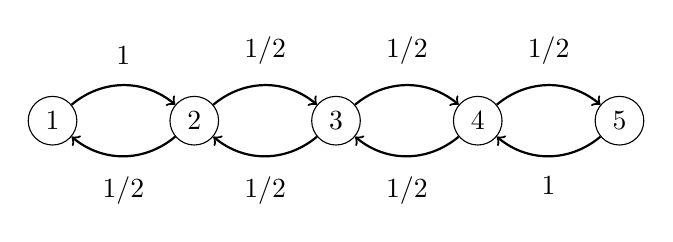
\begin{tikzpicture}[scale=0.9]
\node[draw, circle] (1) at (0,0) {$1$};
\node[draw, circle] (2) at (2,0) {$2$};
\node[draw, circle] (3) at (4,0) {$3$};
\node[draw, circle] (4) at (6,0) {$4$};
\node[draw, circle] (5) at (8,0) {$5$};

\path[draw,thick,->] (1) edge [bend left=40] node[font=\small,label=$1$] {} (2);
\path[draw,thick,->] (2) edge [bend left=40] node[font=\small,label=$1/2$] {} (3);
\path[draw,thick,->] (3) edge [bend left=40] node[font=\small,label=$1/2$] {} (4);
\path[draw,thick,->] (4) edge [bend left=40] node[font=\small,label=$1/2$] {} (5);

\path[draw,thick,->] (5) edge [bend left=40] node[font=\small,label=below:$1$] {} (4);
\path[draw,thick,->] (4) edge [bend left=40] node[font=\small,label=below:$1/2$] {} (3);
\path[draw,thick,->] (3) edge [bend left=40] node[font=\small,label=below:$1/2$] {} (2);
\path[draw,thick,->] (2) edge [bend left=40] node[font=\small,label=below:$1/2$] {} (1);

%\path[draw,thick,->] (1) edge [bend left=40] node[font=\small,label=below:$1$] {} (2);
\end{tikzpicture}
\end{center}

Markovin ketjun tilajakauma on vektori
$[p_1,p_2,\ldots,p_n]$, missä $p_k$ tarkoittaa
todennäköisyyttä olla tällä hetkellä tilassa $k$.
Todennäköisyyksille pätee aina $p_1+p_2+\cdots+p_n=1$.

Esimerkissä jakauma on ensin $[1,0,0,0,0]$,
koska on varmaa, että kulku alkaa kerroksesta 1.
Seuraava jakauma on $[0,1,0,0,0]$,
koska kerroksesta 1 pääsee vain kerrokseen 2.
Tämän jälkeen on mahdollisuus mennä joko ylöspäin
tai alaspäin, joten seuraava jakauma on $[1/2,0,1/2,0,0]$, jne.

Tehokas tapa simuloida kulkua Markovin ketjussa
on käyttää dynaamista ohjelmointia.
Ideana on pitää yllä tilajakaumaa
ja käydä joka vuorolla läpi kaikki tilat
ja jokaisesta tilasta kaikki mahdollisuudet jatkaa eteenpäin.
Tätä menetelmää käyttäen $m$ askeleen simulointi
vie aikaa $O(n^2 m)$.

Markovin ketjun tilasiirtymät voi esittää myös matriisina,
jonka avulla voi päivittää tilajakaumaa askeleen eteenpäin.
Tässä tapauksessa matriisi on

\[ 
 \begin{bmatrix}
  0 & 1/2 & 0 & 0 & 0 \\
  1 & 0 & 1/2 & 0 & 0 \\
  0 & 1/2 & 0 & 1/2 & 0 \\
  0 & 0 & 1/2 & 0 & 1 \\
  0 & 0 & 0 & 1/2 & 0 \\
 \end{bmatrix}.
\]

Tällaisella matriisilla voi kertoa tilajakaumaa esittävän
vektorin, jolloin saadaan tilajakauma yhtä askelta myöhemmin.
Esimerkiksi jakaumasta $[1,0,0,0,0]$ pääsee jakaumaan
$[0,1,0,0,0]$ seuraavasti:

\[ 
 \begin{bmatrix}
  0 & 1/2 & 0 & 0 & 0 \\
  1 & 0 & 1/2 & 0 & 0 \\
  0 & 1/2 & 0 & 1/2 & 0 \\
  0 & 0 & 1/2 & 0 & 1 \\
  0 & 0 & 0 & 1/2 & 0 \\
 \end{bmatrix}
 \begin{bmatrix}
  1 \\
  0 \\
  0 \\
  0 \\
  0 \\
 \end{bmatrix}
=
 \begin{bmatrix}
  0 \\
  1 \\
  0 \\
  0 \\
  0 \\
 \end{bmatrix}.
\]

Matriisiin voi soveltaa edelleen tehokasta
matriisipotenssia, jonka avulla voi laskea
ajassa $O(n^3 \log m)$,
mikä on jakauma $m$ askeleen jälkeen.

\section{Satunnaisalgoritmit}

\index{satunnaisalgoritmi@satunnaisalgoritmi}

Joskus tehtävässä voi hyödyntää satunnaisuutta,
vaikka tehtävä ei itsessään liittyisi todennäköisyyteen.
\key{Satunnaisalgoritmi} on algoritmi, jonka toiminta
perustuu satunnaisuuteen.

\index{Monte Carlo -algoritmi}

\key{Monte Carlo -algoritmi} on satunnaisalgoritmi,
joka saattaa tuottaa joskus väärän tuloksen.
Jotta algoritmi olisi käyttökelpoinen,
väärän vastauksen todennäköisyyden tulee olla pieni.

\index{Las Vegas -algoritmi}

\key{Las Vegas -algoritmi} on satunnaisalgoritmi,
joka tuottaa aina oikean tuloksen mutta jonka
suoritusaika vaihtelee satunnaisesti.
Tavoitteena on, että algoritmi toimisi nopeasti
suurella todennäköisyydellä.

Tutustumme seuraavaksi kolmeen esimerkkitehtävään,
jotka voi ratkaista satunnaisuuden avulla.

\subsubsection{Järjestystunnusluku}

\index{järjestystunnusluku}

Taulukon $k$. \key{järjestystunnusluku}
on kohdassa $k$ oleva alkio,
kun alkiot järjestetään
pienimmästä suurimpaan.
On helppoa laskea mikä tahansa
järjestystunnusluku ajassa $O(n \log n)$
järjestämällä taulukko,
mutta onko oikeastaan tarpeen järjestää koko taulukkoa?

Osoittautuu, että järjestystunnusluvun
voi etsiä satunnaisalgoritmilla ilman taulukon
järjestämistä.
Algoritmi on Las Vegas -tyyppinen:
sen aikavaativuus on yleensä $O(n)$,
mutta pahimmassa tapauksessa $O(n^2)$.

Algoritmi valitsee taulukosta satunnaisen alkion $x$
ja siirtää $x$:ää pienemmät alkiot
taulukon vasempaan osaan ja loput alkiot
taulukon oikeaan osaan.
Tämä vie aikaa $O(n)$, kun taulukossa on $n$ alkiota.
Oletetaan, että vasemmassa osassa on $a$
alkiota ja oikeassa osassa on $b$ alkiota.
Nyt jos $a=k-1$, alkio $x$ on haluttu alkio.
Jos $a>k-1$, etsitään rekursiivisesti
vasemmasta osasta, mikä on kohdassa $k$ oleva alkio.
Jos taas $a<k-1$, etsitään rekursiivisesti
oikeasta osasta, mikä on kohdassa $k-a-1$ oleva alkio.
Haku jatkuu vastaavalla tavalla rekursiivisesti,
kunnes haluttu alkio on löytynyt.

Kun alkiot $x$ valitaan satunnaisesti,
taulukon koko suunnilleen puolittuu
joka vaiheessa, joten kohdassa $k$ olevan
alkion etsiminen vie aikaa
\[n+n/2+n/4+n/8+\cdots=O(n).\]

Algoritmin pahin tapaus on silti $O(n^2)$,
koska on mahdollista,
että $x$ valitaan sattumalta aina niin,
että se on taulukon pienin alkio.
Silloin taulukko pienenee joka vaiheessa
vain yhden alkion verran.
Tämän todennäköisyys on kuitenkin erittäin pieni,
eikä näin tapahdu käytännössä.

\subsubsection{Matriisitulon tarkastaminen}

\index{matriisitulo@matriisitulo}

Seuraava tehtävämme on \emph{tarkastaa},
päteekö matriisitulo $AB=C$, kun $A$, $B$ ja $C$
ovat $n \times n$ -kokoisia matriiseja.
Tehtävän voi ratkaista laskemalla matriisitulon
$AB$ (perusalgoritmilla ajassa $O(n^3)$), mutta voisi toivoa,
että ratkaisun tarkastaminen olisi helpompaa
kuin sen laskeminen alusta alkaen uudestaan.

Osoittautuu, että tehtävän voi ratkaista
Monte Carlo -algoritmilla,
jonka aikavaativuus on vain $O(n^2)$.
Idea on yksinkertainen: valitaan satunnainen
$n \times 1$ -matriisi $X$ ja lasketaan
matriisit $ABX$ ja $CX$.
Jos $ABX=CX$, ilmoitetaan, että $AB=C$,
ja muuten ilmoitetaan, että $AB \neq C$.

Algoritmin aikavaativuus on $O(n^2)$,
koska matriisien $ABX$ ja $CX$ laskeminen
vie aikaa $O(n^2)$.
Matriisin $ABX$ tapauksessa laskennan
voi suorittaa osissa $A(BX)$, jolloin riittää
kertoa kahdesti $n \times n$- ja $n \times 1$-kokoiset
matriisit.

Algoritmin heikkoutena on, että on pieni mahdollisuus,
että algoritmi erehtyy, kun se ilmoittaa, että $AB=C$.
Esimerkiksi 
\[
 \begin{bmatrix}
  2 & 4 \\
  1 & 6 \\
 \end{bmatrix}
\neq
 \begin{bmatrix}
  0 & 5 \\
  7 & 4 \\
 \end{bmatrix},
\]
mutta
\[
 \begin{bmatrix}
  2 & 4 \\
  1 & 6 \\
 \end{bmatrix}
 \begin{bmatrix}
  1 \\
  3 \\
 \end{bmatrix}
=
 \begin{bmatrix}
  0 & 5 \\
  7 & 4 \\
 \end{bmatrix}
 \begin{bmatrix}
  1 \\
  3 \\
 \end{bmatrix}.
\]
Käytännössä erehtymisen todennäköisyys on kuitenkin
pieni ja todennäköisyyttä voi pienentää lisää
tekemällä tarkastuksen usealla
satunnaisella matriisilla $X$ ennen vastauksen
$AB=C$ ilmoittamista.

\subsubsection{Verkon värittäminen}

\index{vxritys@väritys}

Annettuna on verkko, jossa on $n$ solmua ja $m$ kaarta.
Tehtävänä on etsiä tapa värittää verkon solmut kahdella värillä
niin, että ainakin $m/2$ kaaressa
päätesolmut ovat eri väriset.
Esimerkiksi verkossa
\begin{center}
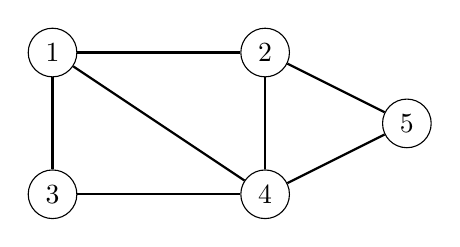
\begin{tikzpicture}[scale=0.9]
\node[draw, circle] (1) at (1,3) {$1$};
\node[draw, circle] (2) at (4,3) {$2$};
\node[draw, circle] (3) at (1,1) {$3$};
\node[draw, circle] (4) at (4,1) {$4$};
\node[draw, circle] (5) at (6,2) {$5$};

\path[draw,thick,-] (1) -- (2);
\path[draw,thick,-] (1) -- (3);
\path[draw,thick,-] (1) -- (4);
\path[draw,thick,-] (3) -- (4);
\path[draw,thick,-] (2) -- (4);
\path[draw,thick,-] (2) -- (5);
\path[draw,thick,-] (4) -- (5);
\end{tikzpicture}
\end{center}
yksi kelvollinen väritys on seuraava:
\begin{center}
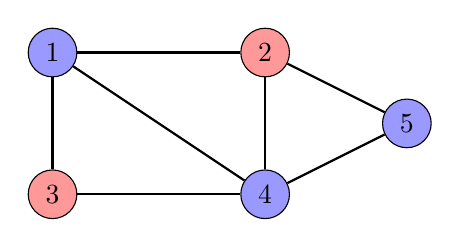
\begin{tikzpicture}[scale=0.9]
\node[draw, circle, fill=blue!40] (1) at (1,3) {$1$};
\node[draw, circle, fill=red!40] (2) at (4,3) {$2$};
\node[draw, circle, fill=red!40] (3) at (1,1) {$3$};
\node[draw, circle, fill=blue!40] (4) at (4,1) {$4$};
\node[draw, circle, fill=blue!40] (5) at (6,2) {$5$};

\path[draw,thick,-] (1) -- (2);
\path[draw,thick,-] (1) -- (3);
\path[draw,thick,-] (1) -- (4);
\path[draw,thick,-] (3) -- (4);
\path[draw,thick,-] (2) -- (4);
\path[draw,thick,-] (2) -- (5);
\path[draw,thick,-] (4) -- (5);
\end{tikzpicture}
\end{center}
Yllä olevassa verkossa on 7 kaarta ja niistä 5:ssä
päätesolmut ovat eri väriset,
joten väritys on kelvollinen.

Tehtävä on mahdollista ratkaista Las Vegas -algoritmilla
muodostamalla satunnaisia värityksiä niin kauan,
kunnes syntyy kelvollinen väritys.
Satunnaisessa värityksessä jokaisen solmun väri on
valittu toisistaan riippumatta niin,
että kummankin värin todennäköisyys on $1/2$.

Satunnaisessa värityksessä todennäköisyys, että yksittäisen kaaren päätesolmut
ovat eri väriset on $1/2$. Niinpä odotusarvo, monessako kaaressa
päätesolmut ovat eri väriset, on $1/2 \cdot m = m/2$.
Koska satunnainen väritys on odotusarvoisesti kelvollinen,
jokin kelvollinen väritys löytyy käytännössä nopeasti.

